\documentclass[11pt]{article}
\usepackage{acl}
\usepackage{times}
\usepackage{latexsym}
\usepackage[T1]{fontenc}
\usepackage[utf8]{inputenc}
\usepackage{microtype}
\usepackage{graphicx}
\usepackage{booktabs}
\usepackage{amsmath}
\usepackage{array}
\usepackage{xcolor}
\usepackage{listings}
\usepackage{enumitem}
\usepackage{url}

\title{BioSciReview-Bench: Benchmarking Coding Agents on\\Silent Scientific Bug Detection in Bioinformatics Code}
\author{Junhao Qiu \\
  Independent Researcher \\
  \texttt{chiujunhao@gmail.com}}

\newcommand{\bench}{\textsc{BioSciReview-Bench}}
\newcommand{\locpm}{Loc@$\pm$3}
\newcommand{\diagpm}{Diagnosis@$\pm$3}
\newcommand{\diagexact}{Diagnosis@Exact}

\lstset{
  basicstyle=\ttfamily\scriptsize,
  breaklines=true,
  numbers=left,
  numberstyle=\tiny\color{gray},
  frame=none,
  xleftmargin=2.2em,
  numbersep=6pt,
  showstringspaces=false,
  keywordstyle=\color{blue},
  commentstyle=\color{gray},
  aboveskip=0.5\baselineskip,
  belowskip=0.5\baselineskip,
}

\begin{document}
\maketitle

\begin{abstract}
Existing coding-agent benchmarks test functional correctness---whether code runs and returns expected outputs. Silent scientific methodology bugs pose a different challenge: they execute without error yet produce plausible, scientifically wrong results. We introduce \bench, a benchmark of 200 manually reviewed synthetic bioinformatics code snippets (100 matched correct--buggy pairs) spanning five domains and six bug categories. Each snippet is presented in isolation without construction metadata; agents must detect whether a bug exists, localize it to a specific displayed line, and classify it by type. We evaluate six configurations across three model families and two agent harnesses. All achieve detection F1 of 0.94--0.99, but performance drops with stricter requirements: joint localization within three lines reaches 0.92--0.98~F1, and full diagnosis requiring exact line plus correct category falls to 0.74--0.89~F1, a gap of approximately 10--23 percentage points below detection. Filtering and quality-control bugs have the lowest average Full Diagnosis@$\pm$3 success rate, and agents sometimes confuse them with normalization errors. Detection performance is high on this controlled benchmark, while delivering actionable diagnoses remains substantially harder.
\end{abstract}

\section{Introduction}

Computational biology depends on complex analysis pipelines where a single methodological error---applying the wrong normalization, omitting a multiple-testing correction, or leaking test labels into training features---can silently propagate through downstream results. Unlike functional bugs that crash or produce obviously wrong output, these silent scientific methodology bugs execute successfully and generate results that look reasonable, making them difficult for both humans and automated systems to catch. As bioinformatics analyses grow in complexity and scale, the cost of undetected methodology errors increases correspondingly \citep{baker2016reproducibility}.

Coding agents powered by large language models have demonstrated strong performance on software engineering tasks \citep{jimenez2024swebench, yang2024sweagent}, suggesting potential as automated code reviewers for scientific software. However, existing benchmarks test agents against functional correctness---resolving GitHub issues, passing test suites, or generating code that compiles and returns correct outputs \citep{chen2021humaneval, austin2021program, hendrycks2021apps}. These tasks provide clear oracles: a failing test or a wrong return value signals the bug. Silent methodology bugs lack such oracles: the code runs, the output has the right shape and type, and determining whether the result is scientifically valid requires domain reasoning about statistical assumptions, experimental design, and biological plausibility.

We introduce \bench, a benchmark that directly tests this capability. The benchmark consists of 200 manually reviewed synthetic bioinformatics code snippets organized as 100 matched pairs: each pair contains a methodologically correct snippet and a corresponding buggy variant that introduces exactly one silent methodology error. Snippets span five bioinformatics domains (bulk RNA-seq, single-cell analysis, variant genomics, clinical/genomic ML, and statistical genomics) and six bug categories (incorrect normalization, wrong statistical test, missing multiple-testing correction, sample mismatch, data leakage, and incorrect filtering). The evaluation is structured as a multi-level hierarchy: agents must first detect whether a bug exists, then localize it to a specific rendered line, and finally classify it by category.

We evaluate six coding-agent configurations spanning three backend families and two harnesses. All agents achieve detection F1 between 0.94 and 0.99. But performance declines progressively as the task demands more actionable output: joint localization within three lines reaches 0.92--0.98 F1, full diagnosis with approximate localization reaches 0.87--0.96 F1, and full diagnosis requiring exact line identification drops to 0.74--0.89 F1. The gap between detection and exact diagnosis ranges from approximately 10 to 23 percentage points depending on the agent: the hard part of scientific code review is not recognizing that something is wrong, but pinpointing exactly what and where.

\section{Related Work}

\paragraph{Code review and bug detection benchmarks.}
SWE-bench \citep{jimenez2024swebench} and agent frameworks built on it \citep{yang2024sweagent} evaluate agents on resolving real GitHub issues, primarily functional bugs with test-suite oracles. CodeReviewer \citep{li2022codereviewer} and related work \citep{tufano2024code} study automated code review but focus on style, maintainability, and general defects rather than scientific correctness. HumanEval \citep{chen2021humaneval}, MBPP \citep{austin2021program}, and APPS \citep{hendrycks2021apps} test code generation against functional specifications. These benchmarks share a reliance on execution-based oracles; \bench\ targets bugs that pass execution and require domain-level reasoning to identify.

\paragraph{Scientific code quality and reproducibility.}
Reproducibility problems are widely documented across science \citep{baker2016reproducibility, ioannidis2005false}. In bioinformatics, prior work has examined reproducibility risks in genomic analyses \citep{baykal2024genomic} and documented spreadsheet-induced gene-name corruption in published data \citep{ziemann2016gene}. However, to our knowledge, no systematic benchmark evaluates AI systems on their ability to detect a broad range of silent methodology bugs directly in scientific code.

\paragraph{Agent evaluation.}
Recent work has expanded agent evaluation beyond single-turn code generation to multi-step task completion \citep{liu2024agentbench, xie2024osworld, zhou2024webarena}, tool use \citep{schick2023toolformer, patil2023gorilla}, and domain-specific applications. \bench\ contributes to this direction by evaluating agents as scientific code reviewers, a setting that requires both programming competence and domain expertise.

\section{\bench}

\subsection{Task Definition}

Given a single bioinformatics code snippet and a statement of its scientific intent (e.g., ``normalize count-like feature measurements and identify high-variance features''), an agent must produce a structured JSON response containing: (1) \textbf{Detection}: whether a scientific methodology bug is present; (2) \textbf{Localization}: the displayed rendered line number of the root cause; (3) \textbf{Classification}: the closest bug category (B1--B6 or null); and (4) \textbf{Rationale}: a concise natural-language explanation. Agents receive no information about whether other snippets exist, whether the current snippet is expected to be correct or buggy, or what distribution of labels to expect. Rationales are retained for qualitative analysis but are not scored.

\subsection{Bug Taxonomy}

The taxonomy covers six categories of silent scientific methodology bugs commonly encountered in bioinformatics pipelines:
\begin{description}[leftmargin=1.2em,style=nextline,noitemsep]
\item[B1 Incorrect normalization, scaling, or transformation.] Applying log-transformation to pre-normalized data, using wrong size factors, or normalizing on raw counts when the method expects CPM.
\item[B2 Wrong statistical test.] Using a parametric test on non-normal data, applying an unpaired test to paired samples, or choosing a correlation method inappropriate for the data distribution.
\item[B3 Missing or incorrect multiple-testing correction.] Omitting FDR adjustment when testing thousands of genes, or applying an inappropriate correction procedure.
\item[B4 Sample mismatch, label swap, or metadata merge error.] Joining expression and phenotype tables on misaligned keys, swapping treatment and control group labels, or assigning outcomes to wrong samples.
\item[B5 Information leakage between training and evaluation data.] Fitting a scaler or selecting features on the full dataset before splitting, or including test-set samples in cross-validation folds.
\item[B6 Incorrect filtering, thresholding, or quality-control criteria.] Using wrong QC cutoffs, applying hard thresholds where adaptive ones are needed, or filtering on the wrong metric.
\end{description}

\subsection{Domain Coverage}

Snippets are drawn from five bioinformatics domains, each represented by 20 pairs (40 snippets): D1 bulk RNA-seq differential expression, D2 single-cell RNA-seq analysis, D3 variant calling and genomic annotation, D4 clinical/genomic machine learning, and D5 statistical genomics (GWAS, eQTL, population genetics). The dataset is balanced across languages: 50 pairs in Python and 50 in R. Bug categories are distributed near-uniformly, with 15--18 instances each.

\subsection{Snippet Construction}

Each benchmark item begins with a synthetic, methodologically correct code snippet implementing a realistic bioinformatics task. We then create a matched buggy variant by introducing exactly one silent methodology error from the six-category taxonomy in Section~3.2. The taxonomy was informed in part by prior work on reproducibility risks and documented data-handling failures in bioinformatics \citep{baykal2024genomic, ziemann2016gene}; all pairs are manually reviewed before inclusion. The buggy variant preserves the same variable names, data structures, imports, and overall code organization; only the lines constituting or immediately surrounding the bug differ. Both snippets in a pair execute without error and produce plausible output, but the buggy variant's output is scientifically invalid.

Annotations record the bug category, the source line containing the root cause, and the expected scientific consequence. Manual quality review checked that (i) each correct snippet is methodologically defensible for its stated intent, (ii) each buggy snippet contains exactly one intended silent bug, and (iii) no snippet contains unintentional methodology issues that could confound evaluation.


Before evaluation, snippets are rendered into a construction-metadata-free view. Maintainer annotations and construction-only inline markers are removed while ordinary scientific comments and docstrings are preserved. Gold root-cause line numbers are remapped to the displayed rendered line numbers, and buggy samples whose gold line maps to no rendered line are rejected. Rendered files use neutral filenames (\texttt{snippet.py} or \texttt{snippet.R}) and random identifiers rather than original paths.

\section{Evaluation Metrics}

We report a hierarchy of F1 metrics over the full 200-snippet evaluation set (100 correct, 100 buggy), plus conditional diagnostic accuracies. \textbf{Detection F1} is binary classification of whether a bug is present. Precision and recall are computed from the $2\times2$ confusion matrix over bug-present predictions.

\textbf{Joint Localization F1} requires both correct detection and localization of the root-cause line. Joint Loc@Exact requires the predicted line to match the gold rendered line exactly. Joint Loc@$\pm$3 allows the predicted line to fall within three rendered lines of the gold line, accommodating cases where the bug's effect is diffuse across adjacent lines. On shorter snippets this tolerance covers a substantial fraction of the program, so Loc@$\pm$3 should be read as ``correct neighborhood'' rather than precise localization. Joint localization does not require the category to be correct.

\textbf{Full Diagnosis F1} requires correct detection, localization, and bug category classification. Full Diagnosis@$\pm$3 combines $\pm$3 localization with correct category. Full Diagnosis@Exact combines exact localization with correct category and is the strictest metric.

For joint localization and full diagnosis, a buggy snippet that is detected but fails the required localization or category condition is counted as both a false positive diagnosis and a false negative gold diagnosis; a correct snippet predicted as buggy is counted as a false positive. This convention treats a wrong diagnosis as both an unsupported claim and a missed gold diagnosis.

\textbf{Conditional accuracy} isolates component ability from detection performance. Conditional Loc@$\pm$3 Accuracy is the fraction of correctly detected buggy snippets with a line prediction that are localized within $\pm$3 lines. Category Accuracy is the fraction of correctly detected buggy snippets with a category prediction that have the correct category.

\textbf{Uncertainty estimation.} Bootstrap 95\% confidence intervals resample at the pair level: each bootstrap sample draws 100 pairs with replacement and includes both snippets from each sampled pair. We recompute all metrics through the unified scorer with 10,000 bootstrap samples per agent.

\section{Experimental Setup}

\subsection{Agent Configurations}

We evaluate six coding-agent configurations spanning three backend model families and two agent harnesses. Two configurations pair Codex CLI with GPT-5.4 and GPT-5.5. Four pair Claude Code (CC) with backend models: Sonnet 4.6, Opus 4.8, DeepSeek-V4-Flash-Preview, and DeepSeek-V4-Pro-Preview (the latter two accessed via an Anthropic-compatible gateway). The two harnesses differ in how they manage file I/O, context presentation, and tool invocation patterns; the evaluated unit is the full agent configuration (harness plus backend model), not the model in isolation. Each agent receives the same prompt template and JSON output schema.

\subsection{Evaluation Procedure}

For each of the 200 rendered snippets, we create a single-sample workspace and invoke the agent once. The workspace contains only four files: the rendered snippet, a task prompt with numbered source lines, the JSON output schema, and a workspace README. It contains no annotations, manifests, paired snippets, project files, or original filenames. Agents are invoked without project-level memory, persistent configuration, browsing, external repositories, or execution-based debugging. The prompt states the scientific intent, defines the six bug categories, and requests a JSON response conforming to the prediction schema; agents are not asked to edit code, run tests, or synthesize patches. Automated checks verify the rendered inputs, workspace contents, and run metadata before scoring. All six agents completed all 200 predictions with zero parse or schema errors.

\section{Results}

\subsection{Main Results}

Table~\ref{tab:main} presents the main results.

\paragraph{Detection performance is high.}
On this controlled benchmark, all six agents achieve detection F1 between 0.943 and 0.990. Recall is at or near 1.0 for every agent; only CC Opus 4.8 and DeepSeek-V4-Flash-Preview each miss a single buggy snippet. The dominant detection error mode is false positives: CC Sonnet 4.6 generates 12 false positives (flagging correct snippets as buggy), while CC Opus 4.8 produces only 1. In short, the evaluated agents rarely miss an injected bug; they over-flag rather than under-flag.

\paragraph{Performance degrades from detection to diagnosis.}
Figure~\ref{fig:cascade} shows the degradation cascade across all four metric levels. The gap between detection F1 and Full Diagnosis@Exact F1 ranges from approximately 10 percentage points (Codex GPT-5.5) to 23 percentage points (DeepSeek-V4-Pro-Preview). Codex GPT-5.5 has the highest reported Full Diagnosis@Exact F1, but its F1 still drops from 0.985 for detection to 0.887 for exact diagnosis. The degradation is progressive: each additional requirement (localization, then category correctness, then exact-line precision) adds incremental difficulty.

\paragraph{Detection and exact diagnosis rankings diverge.}
CC Opus 4.8 achieves the highest detection F1 (0.990), but its Full Diagnosis@Exact F1 drops to 0.760, trailing Codex GPT-5.5 and Codex GPT-5.4 despite stronger detection. It produces 17 near-miss localizations that fall within $\pm$3 lines but miss the exact root-cause line. Codex GPT-5.5 has the highest reported value for every downstream metric in Table~\ref{tab:main}, although its detection F1 is slightly lower. In this evaluation, detection ranking does not match localization or exact-diagnosis ranking.

\begin{table*}[t]
\centering
\small
\begin{tabular}{lcccccc}
\toprule
\textbf{Agent} & \textbf{Detect P/R/F1} & \textbf{FP/FN} & \textbf{Loc@$\pm$3 F1} & \textbf{Diag@$\pm$3 F1} & \textbf{Diag@Exact F1} & \textbf{Cat. Acc.} \\
\midrule
Codex + GPT-5.4 & .962 / 1.00 / .980 & 4 / 0 & .951 & .922 & .814 & .97 \\
Codex + GPT-5.5 & .971 / 1.00 / .985 & 3 / 0 & .975 & .956 & .887 & .98 \\
CC + Sonnet 4.6 & .893 / 1.00 / .943 & 12 / 0 & .915 & .887 & .792 & .97 \\
CC + Opus 4.8 & .990 / .990 / .990 & 1 / 1 & .960 & .930 & .760 & .97 \\
CC + DS-V4-Flash-Prev. & .952 / .990 / .971 & 5 / 1 & .931 & .873 & .775 & .94 \\
CC + DS-V4-Pro-Prev. & .943 / 1.00 / .971 & 6 / 0 & .942 & .883 & .738 & .94 \\
\bottomrule
\end{tabular}
\caption{Main results on \bench. CC = Claude Code. Codex = Codex CLI. Loc@$\pm$3 = Joint Localization within three rendered lines. Diag@$\pm$3 and Diag@Exact = Full Diagnosis requiring localization ($\pm$3 or exact) plus correct bug category. Cat. Acc. = category accuracy among correctly detected buggy snippets.}
\label{tab:main}
\end{table*}

\begin{figure*}[t]
\centering
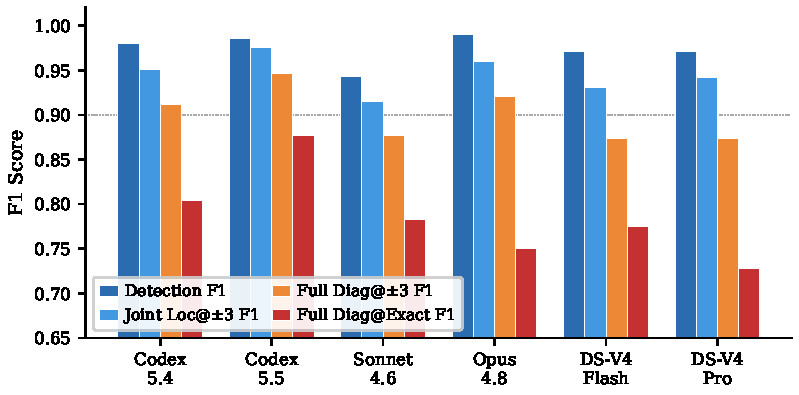
\includegraphics[width=0.85\textwidth]{figs/fig_metric_cascade.pdf}
\caption{Performance degradation cascade. All agents achieve high detection performance but degrade progressively as the task requires localization and classification. The gap between detection and exact diagnosis ranges from approximately 10 to 23 percentage points.}
\label{fig:cascade}
\end{figure*}

\subsection{Bootstrap Confidence Intervals}

Appendix Table~\ref{tab:fullci} reports 95\% pair-level bootstrap confidence intervals for key metrics; here we highlight detection and exact diagnosis. Confidence intervals reflect item-sampling variance only; each agent was queried once per snippet, so run-to-run generation variance is not captured. Detection F1 confidence intervals are narrow, whereas Full Diagnosis@Exact intervals are wider. Codex GPT-5.5 and CC Opus 4.8 have overlapping intervals for detection ([0.97, 1.00] for both) and exact diagnosis ([0.82, 0.95] vs.\ [0.67, 0.84]). The observed point estimates therefore produce different detection and exact-diagnosis rankings, but the intervals overlap and do not capture run-to-run generation variance.


\subsection{Per-Category Analysis}

Figure~\ref{fig:heatmap} shows Full Diagnosis@$\pm$3 success rates broken down by bug category. Performance varies substantially across categories. Multiple-testing correction errors (B3) and data leakage (B5) are diagnosed at or near 100\% by all agents. These categories tend to involve well-known patterns, such as missing \texttt{p.adjust} calls or fitting a scaler before splitting, with strong lexical signals in the code.

Filtering and QC errors (B6) are the most challenging, with success rates as low as 0.71 for DeepSeek-V4-Flash-Preview. Agents frequently misclassify B6 bugs as B1 (normalization), consistent with conceptual overlap between filtering thresholds and scaling operations. Wrong statistical test errors (B2) also prove difficult, with a 0.87--0.93 range across agents.

\begin{figure}[t]
\centering
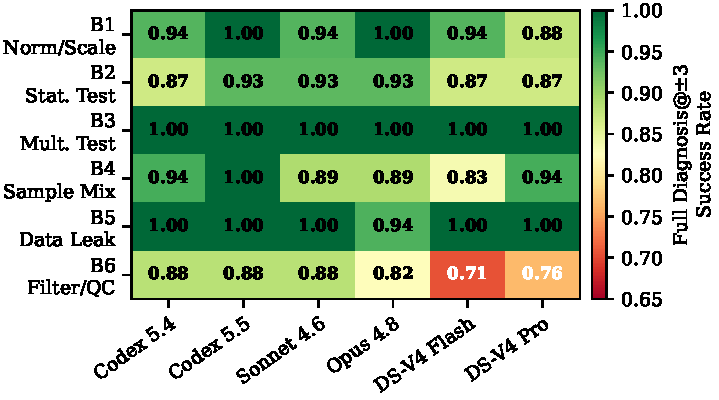
\includegraphics[width=\columnwidth]{figs/fig_category_heatmap.pdf}
\caption{Full Diagnosis@$\pm$3 success rate by bug category and agent. B3 (multiple-testing) and B5 (data leakage) are near-perfectly diagnosed by all agents, while B6 (filtering/QC) is the most challenging.}
\label{fig:heatmap}
\end{figure}

\paragraph{Category confusion patterns.}
Figure~\ref{fig:confusion} shows the aggregate confusion matrix across all agents. Cells show mean per-agent proportions after assigning zero mass to absent off-diagonal categories, so each gold-category row sums to one before rounding. The dominant off-diagonal entries are B6$\to$B1 (13\% of B6 cases) and B4$\to$B1 (6\%). These confusions suggest that agents default to normalization-related explanations when the true error involves boundary-condition or sample-handling reasoning.

\begin{figure}[t]
\centering
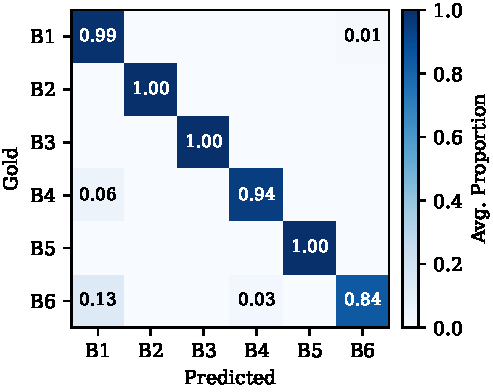
\includegraphics[width=0.85\columnwidth]{figs/fig_category_confusion.pdf}
\caption{Bug category confusion matrix averaged across all six agents. Cells show mean per-agent proportions among detected buggy cases for each gold category, with missing off-diagonal cells treated as zero before averaging. B6$\to$B1 is the dominant misclassification.}
\label{fig:confusion}
\end{figure}

\subsection{Per-Domain and Per-Language Analysis}

Variant genomics (D3) is the most challenging domain for detection, with three agents showing precision below 0.95 due to false positives. This domain features code patterns involving allele-frequency calculations and multi-allelic variant handling where defensible methodological choices can appear suspicious. Bulk RNA-seq (D1) and statistical genomics (D5) are the easiest domains for localization, likely because their analysis patterns follow well-established conventions.

Performance is comparable across Python and R, though R snippets show slightly higher detection precision for most agents (e.g., CC Sonnet 4.6 achieves 0.926 precision on R vs. 0.862 on Python).

\subsection{Qualitative Error Analysis}

We examine the 7 buggy snippets where all six agents fail on exact diagnosis to identify systematic failure modes. Three patterns emerge.

\paragraph{Consequence-line errors (4 cases).}
Four B3 snippets (missing multiple-testing correction) produce identical off-by-one errors across all agents: every agent points to line $N+1$, where the uncorrected $p$-value is used, rather than line $N$, where the correction should have been applied. The agents correctly identify the bug type and localize to within one line, but consistently attribute the root cause to the downstream consequence rather than the upstream omission. This pattern suggests agents reason backward from observed misuse rather than forward from missing operations.

\paragraph{Correct line, wrong category (2 cases).}
Two B6 snippets in variant genomics are localized to the exact line by all agents but uniformly misclassified as B1 (normalization). Both involve allele-frequency denominators that include missing genotypes---a filtering/QC error (denominator should exclude uncalled samples) that agents interpret as a scaling error. The B6$\to$B1 confusion accounts for 13\% of B6 cases across all agents (Figure~\ref{fig:confusion}), and these two cases demonstrate that the confusion is systematic and shared, not model-specific.

\paragraph{Propagation-line errors (1 case).}
One B2 snippet (single-cell pseudoreplication) is correctly classified by all agents but localized 6 lines downstream of the gold root cause. The bug is the definition of the shuffling scope, where cell-level rather than donor-level permutation is specified, but all agents point to the permutation-test execution. The agents identify the correct statistical flaw but attribute it to where the test runs rather than where the flawed scope is defined.

\paragraph{False positives.}
Across all agents, 31 of 600 correct-snippet predictions are false positives (5.2\%). Variant genomics (D3) accounts for a disproportionate share: agents flag defensible methodological choices, such as pooling correction families across panels or retaining technical covariates, as bugs. The rationales are scientifically coherent but reflect a stricter standard than the benchmark's intent, where the correct snippet is defined as methodologically defensible for its stated purpose.

\subsection{Retrospective Best-of-Six Upper Bound}

To quantify complementary coverage across agents, we compute a retrospective best-of-six upper bound: a buggy case is counted as solved if any of the six agents solves it. This calculation uses gold labels after the fact to identify whether at least one agent succeeded, and therefore should not be interpreted as a deployable ensemble.

The best-of-six upper bound reaches 100\% detection recall, 99\% joint localization@$\pm$3, 97\% full diagnosis@$\pm$3, and 93\% full exact diagnosis. The seven cases not solved by any configuration under exact diagnosis are shared failure cases: five involve consequence or propagation lines rather than the annotated root-cause line, and two involve a shared B6$\to$B1 category confusion.

Conversely, the all-agents intersection---cases where every agent succeeds---achieves 98\% detection, 91\% localization, 86\% diagnosis@$\pm$3, and only 69\% exact diagnosis. The gap between the best-of-six upper bound (93\%) and the intersection (69\%) indicates substantial complementarity across agent configurations: different agents succeed on different subsets of the harder cases.

\section{Discussion}

\paragraph{The detection--diagnosis gap.}
Current coding agents are much better at detecting the presence of a methodology bug than at identifying exactly what is wrong and where. Detection recall is 99--100\% across the evaluated configurations, but exact-diagnosis F1 is approximately 10--23 percentage points lower than detection F1. Practitioners therefore still need domain expertise to verify the proposed root cause and category.

\paragraph{Category difficulty reflects conceptual structure.}
The spread across categories is consistent with differences in conceptual structure rather than dataset imbalance. Multiple-testing and data-leakage bugs follow rigid, well-documented patterns with strong lexical cues. Filtering and QC bugs require judgment about domain-appropriate thresholds: what counts as a wrong cutoff depends on context that a short snippet may not fully supply.

\paragraph{Complementary error profiles.}
The best-of-six analysis shows that different agents fail on different cases; ensemble or routing strategies could plausibly narrow the diagnosis gap. These shared failures include both line-attribution and category-boundary errors. Richer pipeline context may help in some cases, but the present experiment does not test that.

\section{Conclusion}

\bench\ provides, to our knowledge, the first benchmark focused on coding-agent diagnosis of silent bioinformatics methodology bugs. Our evaluation of six agent configurations reveals a consistent detection--diagnosis gap: agents can flag buggy code with near-perfect recall but struggle to provide the exact root-cause localization and bug categorization needed for actionable scientific code review. Evaluating scientific coding agents requires moving beyond binary bug detection: actionable review depends on root-cause localization and category-aware diagnosis. The benchmark data and code are available at \url{https://github.com/qchiujunhao/BioSciReview-Bench}.

\section*{Limitations}

The benchmark uses isolated code snippets rather than full analysis pipelines, which simplifies the task relative to real-world code review. Exact-line scoring uses a single annotated root-cause line, although omission and propagation errors may also be localized to an adjacent consequence or execution line. Snippets are manually reviewed synthetic constructions, not extracted from published analyses. The six-category taxonomy, while covering major error types, does not exhaust all possible scientific methodology bugs. We do not evaluate patch generation or execution-based repair; the benchmark targets the diagnostic stage of scientific code review. Patch synthesis is left to future work because silent methodology bugs may admit multiple scientifically valid repairs and often lack executable test oracles. Cross-harness comparisons (Codex CLI vs.\ Claude Code) confound harness and model; rankings within the same harness are more interpretable. All agents received a single prompt template, so sensitivity to prompt phrasing is unmeasured. The agent configurations evaluated here represent a snapshot; rapid model development may shift the performance landscape.

\section*{Ethics Statement}

All code snippets in the benchmark are manually reviewed synthetic constructions and do not contain or derive from patient data, protected health information, or proprietary analysis code. The benchmark is intended for evaluating AI systems and does not constitute medical or scientific advice. We used OpenAI GPT-5.5 (via Codex Desktop) and Anthropic Claude Opus 4.6 (via Claude Desktop) as writing assistants during manuscript preparation; all scientific claims, experimental design, data analysis, and editorial decisions are the author's own.

\begingroup\small
\begin{thebibliography}{99}
\bibitem[Austin et~al.(2021)]{austin2021program} Jacob Austin, Augustus Odena, Maxwell Nye, Maarten Bosma, Henryk Michalewski, David Dohan, Ellen Jiang, Carrie Cai, Michael Terry, Quoc Le, and Charles Sutton. 2021. Program synthesis with large language models. \emph{arXiv preprint arXiv:2108.07732}.
\bibitem[Baker(2016)]{baker2016reproducibility} Monya Baker. 2016. 1,500 scientists lift the lid on reproducibility. \emph{Nature}, 533(7604):452--454.
\bibitem[Baykal et~al.(2024)]{baykal2024genomic} Pelin Icer Baykal, Pawe{\l} Piotr {\L}abaj, Florian Markowetz, Lynn M. Schriml, Daniel J. Stekhoven, Serghei Mangul, and Niko Beerenwinkel. 2024. Genomic reproducibility in the bioinformatics era. \emph{Genome Biology}, 25:213.
\bibitem[Chen et~al.(2021)]{chen2021humaneval} Mark Chen et~al. 2021. Evaluating large language models trained on code. \emph{arXiv preprint arXiv:2107.03374}.
\bibitem[Hendrycks et~al.(2021)]{hendrycks2021apps} Dan Hendrycks et~al. 2021. Measuring coding challenge competence with APPS. In \emph{NeurIPS Datasets and Benchmarks}.
\bibitem[Ioannidis(2005)]{ioannidis2005false} John P. A. Ioannidis. 2005. Why most published research findings are false. \emph{PLoS Medicine}, 2(8):e124.
\bibitem[Jimenez et~al.(2024)]{jimenez2024swebench} Carlos E. Jimenez et~al. 2024. SWE-bench: Can language models resolve real-world GitHub issues? In \emph{ICLR}.
\bibitem[Li et~al.(2022)]{li2022codereviewer} Zhiyu Li, Shuai Lu, Daya Guo, Nan Duan, Shailesh Jannu, Grant Jenks, Deep Majumder, Jared Green, Alexey Svyatkovskiy, Shengyu Fu, and Neel Sundaresan. 2022. Automating code review activities by large-scale pre-training. In \emph{Proceedings of the 30th ACM Joint European Software Engineering Conference and Symposium on the Foundations of Software Engineering}, pages 1035--1047.
\bibitem[Liu et~al.(2024)]{liu2024agentbench} Xiao Liu et~al. 2024. AgentBench: Evaluating LLMs as agents. In \emph{ICLR}.
\bibitem[Patil et~al.(2023)]{patil2023gorilla} Shishir G. Patil, Tianjun Zhang, Xin Wang, and Joseph E. Gonzalez. 2023. Gorilla: Large language model connected with massive APIs. \emph{arXiv preprint arXiv:2305.15334}.
\bibitem[Schick et~al.(2023)]{schick2023toolformer} Timo Schick et~al. 2023. Toolformer: Language models can teach themselves to use tools. In \emph{NeurIPS}.
\bibitem[Tufano et~al.(2024)]{tufano2024code} Rosalia Tufano, Ozren Dabic, Antonio Mastropaolo, Matteo Ciniselli, and Gabriele Bavota. 2024. Code review automation: Strengths and weaknesses of the state of the art. \emph{IEEE Transactions on Software Engineering}, 50(2):338--353.
\bibitem[Xie et~al.(2024)]{xie2024osworld} Tianbao Xie et~al. 2024. OSWorld: Benchmarking multimodal agents for open-ended tasks in real computer environments. In \emph{NeurIPS}.
\bibitem[Yang et~al.(2024)]{yang2024sweagent} John Yang et~al. 2024. SWE-agent: Agent-computer interfaces enable automated software engineering. In \emph{NeurIPS}.
\bibitem[Zhou et~al.(2024)]{zhou2024webarena} Shuyan Zhou et~al. 2024. WebArena: A realistic web environment for building autonomous agents. In \emph{ICLR}.
\bibitem[Ziemann et~al.(2016)]{ziemann2016gene} Mark Ziemann, Yotam Eren, and Assam El-Osta. 2016. Gene name errors are widespread in the scientific literature. \emph{Genome Biology}, 17(1):177.
\end{thebibliography}
\endgroup

\clearpage
\appendix

\section{Prompt Template}
The prompt shown to each agent follows this structure (concrete example abbreviated):
\begin{quote}\small
You are reviewing a single bioinformatics code snippet for silent scientific methodology bugs. The snippet may be methodologically valid or may contain one methodology bug. Bug categories: B1: Incorrect normalization ... [B2--B6 descriptions]. Scientific intent: [task description]. Code: \texttt{1 | import numpy as np} ... Return only JSON matching this schema: \{...\}
\end{quote}

\section{Full Bootstrap Confidence Intervals}
Table~\ref{tab:fullci} provides bootstrap CIs for key metrics.
\begin{table*}[h]
\centering
\small
\resizebox{\textwidth}{!}{%
\begin{tabular}{lccccc}
\toprule
\textbf{Agent} & \textbf{Detect F1} & \textbf{Loc@$\pm$3 F1} & \textbf{Diag@$\pm$3 F1} & \textbf{Diag@Exact F1} & \textbf{Cat. Acc.} \\
\midrule
Codex + GPT-5.4 & .980 [.96, 1.00] & .951 [.91, .99] & .922 [.87, .97] & .814 [.74, .89] & .97 [.93, 1.00] \\
Codex + GPT-5.5 & .985 [.97, 1.00] & .975 [.95, 1.00] & .956 [.91, .99] & .887 [.82, .95] & .98 [.95, 1.00] \\
CC + Sonnet 4.6 & .943 [.91, .97] & .915 [.87, .95] & .887 [.83, .94] & .792 [.72, .86] & .97 [.93, 1.00] \\
CC + Opus 4.8 & .990 [.97, 1.00] & .960 [.92, .99] & .930 [.88, .98] & .760 [.67, .84] & .97 [.93, 1.00] \\
CC + DS-V4-Flash-Prev. & .971 [.95, .99] & .931 [.89, .97] & .873 [.81, .93] & .775 [.70, .85] & .94 [.89, .98] \\
CC + DS-V4-Pro-Prev. & .971 [.95, .99] & .942 [.90, .98] & .883 [.82, .94] & .738 [.65, .82] & .94 [.89, .98] \\
\bottomrule
\end{tabular}}
\caption{95\% bootstrap confidence intervals (10,000 pair-level resamples) for key metrics.}
\label{tab:fullci}
\end{table*}

\section{Per-Category Breakdown}
Table~\ref{tab:percat} reports detection recall and Full Diagnosis@$\pm$3 success rate per category for each agent.
\begin{table*}[h]
\centering
\small
\resizebox{\textwidth}{!}{%
\begin{tabular}{lcccccccccccc}
\toprule
 & \multicolumn{2}{c}{Codex+5.4} & \multicolumn{2}{c}{Codex+5.5} & \multicolumn{2}{c}{CC+Son.4.6} & \multicolumn{2}{c}{CC+Op.4.8} & \multicolumn{2}{c}{CC+DS-Fl.} & \multicolumn{2}{c}{CC+DS-Pro} \\
\cmidrule(lr){2-3}\cmidrule(lr){4-5}\cmidrule(lr){6-7}\cmidrule(lr){8-9}\cmidrule(lr){10-11}\cmidrule(lr){12-13}
\textbf{Cat.} & Rec. & D@3 & Rec. & D@3 & Rec. & D@3 & Rec. & D@3 & Rec. & D@3 & Rec. & D@3 \\
\midrule
B1 (16) & 1.0 & .94 & 1.0 & 1.00 & 1.0 & .94 & 1.0 & 1.00 & .94 & .94 & 1.0 & .88 \\
B2 (15) & 1.0 & .87 & 1.0 & .93 & 1.0 & .93 & 1.0 & .93 & 1.0 & .87 & 1.0 & .87 \\
B3 (17) & 1.0 & 1.00 & 1.0 & 1.00 & 1.0 & 1.00 & 1.0 & 1.00 & 1.0 & 1.00 & 1.0 & 1.00 \\
B4 (18) & 1.0 & .94 & 1.0 & 1.00 & 1.0 & .89 & 1.0 & .89 & 1.0 & .83 & 1.0 & .94 \\
B5 (17) & 1.0 & 1.00 & 1.0 & 1.00 & 1.0 & 1.00 & 1.0 & .94 & 1.0 & 1.00 & 1.0 & 1.00 \\
B6 (17) & 1.0 & .88 & 1.0 & .88 & 1.0 & .88 & .94 & .82 & 1.0 & .71 & 1.0 & .76 \\
\bottomrule
\end{tabular}}
\caption{Per-category detection recall (Rec.) and Full Diagnosis@$\pm$3 success rate (D@3) for each agent. Category counts (number of buggy snippets) shown in parentheses.}
\label{tab:percat}
\end{table*}

\section{Benchmark Examples}
For readability, examples in this appendix mark the bug line with an inline comment; these annotations were added only for exposition and were not present in agent inputs.

\paragraph{Example 1: Data leakage (B5).}
The snippet performs feature selection for a nearest-centroid classifier. Line~15 computes selection scores using the entire dataset, including test samples. The correct version replaces \texttt{features} and \texttt{labels} with \texttt{X\_train} and \texttt{y\_train}, restricting selection to training data.
\begin{lstlisting}[language=Python,firstnumber=10]
train_idx = np.arange(n_train)
test_idx  = np.arange(n_train, n_train + n_test)
X_train, y_train = features[train_idx], labels[train_idx]
X_test,  y_test  = features[test_idx],  labels[test_idx]

selection_scores = np.abs(       # <-- BUG
    features[labels == 1].mean(0)
  - features[labels == 0].mean(0))
selected = np.argsort(selection_scores)[-6:]
\end{lstlisting}

\paragraph{Example 2: Incorrect filtering (B6).}
The snippet filters observations by a quality metric. Line~13 uses \texttt{< 0.60}, retaining low-quality observations and discarding good ones. The correct version uses \texttt{>= 0.60}.
\begin{lstlisting}[language=Python,firstnumber=9]
marker_signal = quality * 2.4 + rng.normal(0, 0.1, n_obs)
qc = pd.DataFrame({"quality": quality,
                   "detected_features": detected_features,
                   "marker_signal": marker_signal})
keep = qc["quality"] < 0.60     # <-- BUG
filtered = qc[keep]
high_marker = (filtered["marker_signal"] > 1.6).sum()
print("Observations retained:", len(filtered))
\end{lstlisting}


\end{document}
